\documentclass{beamer}
\usetheme{Madrid}

%Statement environment
\newcommand{\statement}[1]{\stepcounter{statements}\begin{center}
	\textbf{#1}
	\end{center}
}

%Color Settings
\usepackage{xcolor}
\definecolor{BScRed}{RGB}{157,0,0}
\definecolor{BScBlue}{RGB}{1,1,141}
\definecolor{BScGreen}{RGB}{0, 119, 85}
\definecolor{BScGray}{RGB}{102, 102, 142}

%Useful definitions

\newcommand{\Z}{\mathcal{Z}[J]}
\renewcommand{\S}{\mathcal{S}[\varphi]}
\newcommand{\D}{\mathcal{D}}
\newcommand{\W}{\mathcal{W}[J]}
\newcommand{\cf}[1]{\langle #1 \rangle}


\newcommand{\Ricci}{\mathcal{R}}
\newcommand{\Gammak}{\Gamma_{k}}
%\newcommand{\Gamma2}{\Gamma^{(2)}_{k}}
\newcommand{\Lambdak}{\Lambda_k}
\renewcommand{\tr}[1]{\operatorname{Tr}\left[ #1 \right]}
%Personel Data
\title{Asymptotic safety of gravity-matter systems}
%\subtitle{This is my subtitle}
\author[Mathieu Kaltschmidt]{Mathieu Kaltschmidt}
\institute[ITP Heidelberg]
{
Institute for Theoretical Physics \\
Heidelberg University \\
}

\titlegraphic{
\includegraphics[width=2cm]{figures/signet}\hspace*{2cm}~%
	
\includegraphics[width=2cm]{figures/signet}
}

\date[08. Juli 2019]
{
%Bachelor Thesis Defence \\
July 8th, 2019
}

% Change base colour beamer@blendedblue (originally RGB: 0.2,0.2,0.7)
\colorlet{beamer@blendedblue}{red!55!black}


%Math and Units
\usepackage{amsmath, amssymb, commath, mathtools}
\usepackage{physics}
\usepackage{xfrac}
\usepackage[separate-uncertainty]{siunitx}


%Tables
\usepackage{array} %math mode in tables
\usepackage{booktabs} %hline rules

%Language Settings and Microtype
\usepackage{fontspec, xunicode}
\usepackage[utf8]{inputenc}
\usepackage{lmodern}
\setsansfont{Palatino}
%\setsansfont{Optima}
\setmonofont[Scale=MatchLowercase]{Menlo}
\usepackage{polyglossia}
\setmainlanguage{english}
\setotherlanguages{german, french}
\usepackage{microtype}

%Useful Packages
\usepackage{graphicx} %including images
\usepackage{float} %better positioning for float environments
\usepackage{blindtext} %for testing the output
\usepackage[labelfont=bf]{caption} %nice captions
\usepackage{subcaption} %for multiple plots

\usepackage[
	style=numeric-comp,
	backend=biber,
	isbn=false,
	date=year,
	url=false,
	doi=false,
	hyperref = auto
]{biblatex}
\addbibresource{bsc.bib}
\setbeamertemplate{bibliography item}{\insertbiblabel}

\beamertemplatenavigationsymbolsempty

%Colorlinks etc.
%\usepackage[colorlinks=True]{hyperref}
%\hypersetup{allcolors=BScBlue}
\usepackage{setspace}
\setbeamertemplate{caption}[numbered]
\usepackage{slashed}
\usepackage{subcaption}


\begin{document}
\maketitle

\begin{frame}{Contents}
\begin{columns}
\begin{column}{\textwidth}
{\vspace{-0.5cm}\setstretch{3}
\tableofcontents
}	
\end{column}
\end{columns}
\end{frame}

%Classical Gravity 
\section{Challenge: Finding a Quantum Field Theory for Gravity}
\begin{frame}{General Relativity}
Understanding of gravity is based on the concept of \textbf{curved spacetime}.
\begin{itemize}
	\item Metric tensor, Riemann tensor + contractions
	\begin{align}
	g_{\mu\nu}, \qquad R_{\phantom{\alpha}\beta \gamma \delta}^{\alpha}, \qquad
R_{\mu\nu} = R^{\alpha}_{\phantom{\alpha}\mu\alpha\nu}, \qquad \mathcal{R} = R^{\mu}_{\phantom{\mu}\mu}
\end{align}
	\item Einstein-Hilbert action:
	\begin{align}
	\mathcal{S}_{\text{EH}} = \frac{1}{16\pi G} \int_x \sqrt{g} \ (\mathcal{R} - 2\Lambda) + \text{matter}
	\end{align}
	\item Equations of motion: Einstein's equations
	\begin{align}
	\frac{1}{8\pi G}\left[G_{\mu\nu} + \Lambda g_{\mu\nu}\right] = T_{\mu\nu}	
	\end{align}
	\end{itemize}	
\centering\bfseries\large
But is there a \textit{quantum} theory of gravity?
\end{frame}

\begin{frame}{A Path Integral for Gravity?}
Naive approach: quantizing gravity via the path integral formalism.\\
\vspace{0.3cm}
\begin{itemize}
	\item Introduce linear split in metric:
	\begin{equation}
		g_{\mu\nu} = \bar{g}_{\mu\nu} + \sqrt{G} \ h_{\mu\nu}
	\end{equation}
	\item Path integral representation of quantum gravity:
	\begin{equation}
	Z[J ; \bar{g}]=\int_{\Phi} \operatorname{e}^{-\mathcal{S}_{\text{grav}}\left[\bar{g}_{\mu\nu}, \Phi\right]+\int_x \sqrt{\bar{g}} \ J \cdot \Phi}, \qquad \Phi = \left(h_{\mu\nu},c_{\mu},\bar{c}_{\mu\nu}\right)
	\end{equation}
	\item Analysis of canonical mass dimensions:
	 \begin{equation}
\left[G\right] = \left[\dd^dx \sqrt{g}\ \mathcal{R}\right] = 2-d,  \qquad\qquad \left[\Lambda\right] = 2
\end{equation}
\end{itemize}	
\centering\bfseries\large
$G$ has negative mass dim. in $d=4$ spacetime dimensions.
\end{frame}

\begin{frame}{Perturbative Non-Renormalizability}
\begin{figure}[t]
	\centering
	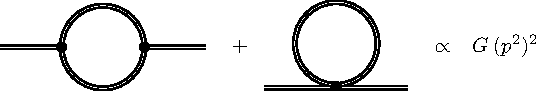
\includegraphics[width=0.8\textwidth]{figures/vacuum_pol}
	\caption{Vacuum polarization diagrams up to $1$-loop order.}
	\hrulefill
\end{figure}
\begin{itemize}
	\item \textbf{t'Hooft \& Veltman:} Theory renormalizable up to 1-loop order. \vspace{0.4cm}
	\item \textbf{Goroff \& Sagnotti:} Non-vanishing counterterms at 2-loop order:
	\begin{equation}
		 S_{\mathrm{GS}}=\frac{1}{\varepsilon} \frac{209}{2880} \frac{1}{(4 \pi)^{4}} \int_x \sqrt{g} \ C_{\mu \nu}^{\phantom{\mu \nu}\kappa \lambda} C_{\kappa \lambda}^{\phantom{\kappa \lambda}\rho \sigma} C_{\rho \sigma}^{\phantom{\rho \sigma}\mu \nu}
		\end{equation}
\end{itemize}
\vspace{0.1cm}
\centering\bfseries\large
Failure of perturbative quantization!	
\end{frame}

%FRG and Flow equation
\section{Method: The Functional Renormalization Group}

\begin{frame}{The Functional Renormalization Group}
\begin{figure}[t]
\centering
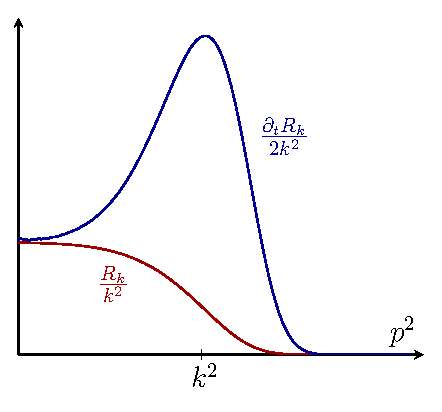
\includegraphics[width=0.35\textwidth]{figures/regulator_plot}
\caption{Shape of a typical exponential regulator function $R(p^2)$ and its\\ \hspace{1.4cm} derivative w.\,r.\,t. the RG time $t = -\ln (k/\Lambda)$.}
\vspace{-0.3cm}
\hrulefill	
\end{figure}
\vspace{-0.3cm}
	\begin{itemize}
		\item \textbf{Idea:} Shell-wise momentum integration to solve path integral\vspace{0.2cm}
		\item  \textbf{Realization:} Introducing IR cutoff scale $k$ via \textbf{regulator}
	\end{itemize}
\end{frame}

\begin{frame}{The Flow Equation}
\vspace{0.6cm}
\begin{itemize}
	\item Interpolation process between $\Gamma_{k\rightarrow\infty}\equiv\mathcal{S}$ and $\Gamma_{k\rightarrow 0}\equiv\Gamma$ governed by Wetterich's flow equation:
\end{itemize}
\begin{block}{Wetterich equation}
\begin{align}
		\partial_t\Gamma_k[\phi] = \frac{1}{2}\operatorname{STr}\bigl[G_k\ \partial_tR_k \bigr], \qquad G_k := \left(\Gamma^{(2)}_k[\phi] + R_k\right)^{-1}_{ji}
	\end{align}	
\end{block}

\begin{itemize}
\item Diagrammatical representation as exact 1-loop equation:
\end{itemize}
\vspace{-0.6cm}
\begin{figure}
	\centering
	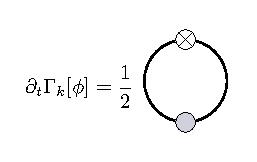
\includegraphics[width=0.5\textwidth]{figures/flow_eqn2}
\end{figure}

\end{frame}
\begin{frame}{Asymptotic Safety}
\begin{figure}
	\centering
	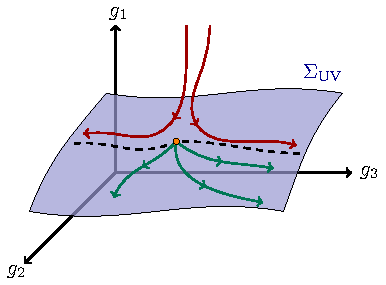
\includegraphics[width=0.45\textwidth]{figures/hypersurface}
	\caption{Visualization of a fixed point $g^*$ and its corresponding UV hyper-\\ \hspace{1.4cm} surface $\Sigma_{\text{UV}}$.}
	\vspace{-0.3cm}
	\hrulefill
\end{figure}
\vspace{-0.2cm}
\begin{enumerate}
	\item Existence of an UV-attractive Non-Gaussian Fixed Point.\vspace{0.3cm}
	\item $\Gamma_k$ fixed by a finite amount of measurements:
	\begin{equation*}
		\operatorname{dim}\Sigma_{\mathrm{UV}} < \infty.
	\end{equation*} 
\end{enumerate} 
\end{frame}

%Pure-Gravity
\section{Results I: Pure-Gravity System}
\begin{frame}{Einstein-Hilbert Truncation}
\begin{itemize}
	\item Simple truncation, takes only $\Lambda$ and $\mathcal{R}$ into account:
	\end{itemize}
\begin{equation}
	\Gamma_k = \frac{Z_{h,k}}{16\pi G} \int_x \sqrt{g} \ [-\mathcal{R} + 2\Lambda_k] + \mathcal{S}_{\text{gf}} + \mathcal{S}_{\text{gh}}
\end{equation}
\begin{itemize}
	\item Left hand side of the flow equation:
\end{itemize}
\begin{equation}
	\partial_{t}\Gamma_{k} = \frac{Z_{h,k}}{16\pi G}\int_x \sqrt{g} \left\{\eta_h\mathcal{R}+2\left(k^2(\partial_t\lambda_k) + \Lambda_k(2 - \eta_h)\right)\right\}
\end{equation}
\begin{itemize}
	\item \textbf{Idea:} Compute the functional trace on the r.\,h.\,s. of the flow equation and compare terms of different orders in $\mathcal{R}$ to obtain the beta functions.
\end{itemize}
\end{frame}

\begin{frame}{Solving the Flow Equation}
\textbf{First.} Background field method and \textit{York decomposition} of the \\ \hspace{0.9cm} fluctuation field $h_{\mu\nu}$:
\begin{equation}
	h_{\mu v}= \structure{h_{\mu v}^{\mathrm{TT}}}+\bar{\nabla}_{\mu} \xi_{v}+\bar{\nabla}_{v} \xi_{\mu}+\left(\bar{\nabla}_{\mu} \bar{\nabla}_{v}-\frac{1}{d} \bar{g}_{\mu v} \bar{\Delta}\right) \sigma+\textcolor{BScGreen}{\frac{1}{d} \bar{g}_{\mu v} h}.
	\label{eqn:York}
\end{equation}
\textbf{Then.} Proceed as follows:\vspace{0.3cm}
\begin{enumerate}
	\item Choose a suitable regulator $R_k$\vspace{0.4cm}
	\item Determine the full propagator $G_k$\vspace{0.4cm}
	\item Compute the scale derivative of the chosen regulator $\partial_tR_k$\vspace{0.4cm}
	\item Make use of \textit{heat-kernel techniques}
\end{enumerate}
	
\end{frame}

\begin{frame}{Beta Functions and Fixed Points}
\begin{itemize}
	\item Beta function for Newtons coupling constant:
	\begin{align}
	\beta_g = \partial_t g_k = \left(2 + \eta_h\right)g_k.
	\label{eqn:beta_gk}
\end{align}
	\item Graviton anomalous dimension:
	\begin{align}
\eta_h = -\frac{5g_k}{3\pi} \left(\frac{1-\frac{\eta_h}{4}}{1-2\lambda_k} + 2\frac{1-\frac{\eta_h}{6}}{(1-2\lambda_k)^2}\right).	
\end{align}
	\item Beta function for the cosmological constant:
	\begin{align}
	\beta_{\lambda} = \partial_t\lambda_k = -4\lambda_k + \frac{\lambda_k}{g_k} \partial_t g_k + \frac{5}{4\pi}g_k\frac{1-\frac{\eta_h}{6}}{1-2\lambda_k}.
\end{align}
\end{itemize}
\end{frame}

\begin{frame}{Phase Diagram}
	\begin{figure}
	\centering
	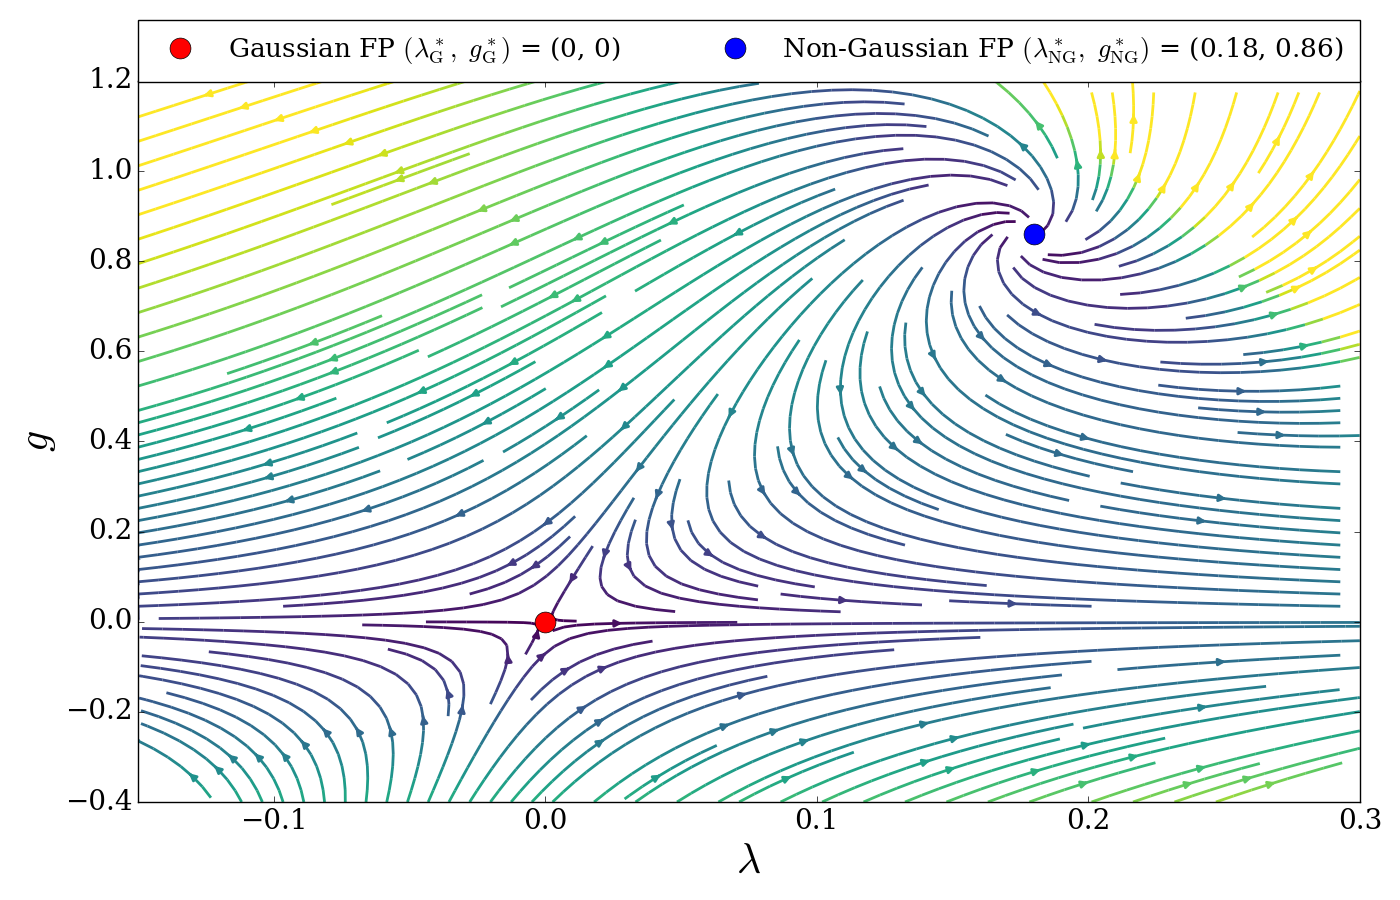
\includegraphics[width=0.8\textwidth]{figures/EH_NoMatter}
	\caption{Flow diagram  for the Einstein-Hilbert truncation in $h^{\mathrm{TT}}$ approxima-\\ \hspace{1.4cm} tion. The flow points towards the infrared.}
\end{figure}
\end{frame}

\begin{frame}{Inclusion of the other Graviton modes}
\begin{itemize}
	\item Gauge fixing choice $\beta=0 , \alpha\rightarrow 0$ leaves us with:
\end{itemize}
\vspace{0.4cm}
\begin{equation} G_{k, h h}= \frac{32\pi}{Z_h}
\begin{pmatrix}
\frac{1}{\bar{\Delta}\left[1+r_{k}\right]-2\Lambda_k+\frac{2}{3}\mathcal{R}} & 0 & 0 & 0 \\[10pt]
0 & 0  & 0 & 0 \\[10pt]
0 & 0 & \frac{-\frac{8}{3}}{\bar{\Delta}\left[1+r_{k}\right]-\frac{4}{3} \Lambda_k}  &0\\[10pt]
0 & 0 & 0 & 0 \\
\end{pmatrix}
\end{equation}
\vspace{0.4cm}
\begin{itemize}
	\item \textbf{Attention:}  New heat-kernel coefficients due to modified Laplacian $\tilde{\Delta} = -\nabla^2 + \mathbf{E}$ occurring in the ghost term!

\end{itemize}
\end{frame}
%Gravity-Matter
\section{Results II: Gravity-Matter Systems}

\begin{frame}{Gravity-Matter systems}
\begin{figure}
	\centering
	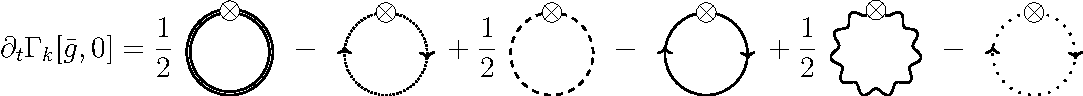
\includegraphics[width=\textwidth]{figures/matter_corrections}
	\caption{Flow equation (\ref{eqn:matter_flow}) for $\Gamma_k$ including different matter contributions in \\
	\hspace{1.4cm} diagrammatic representation.}
	\vspace{-0.2cm}
	\hrulefill
\end{figure}
\begin{itemize}
	\item Inclusion of matter straightforward:
	\vspace{-0.2cm}
	\begin{align}
		\Gamma_k = \Gamma_{\text{EH}} + \mathcal{S}_{\text{gf}} + \mathcal{S}_{\text{gh}} + \overbrace{\mathcal{S}_{S} + \mathcal{S}_{D} + \mathcal{S}_{V}}^{=: \ \Gamma_{\text{matter}}}
	\end{align}
	\item Resulting flow equation:
	\begin{equation}
\begin{aligned}
 \partial_t\Gamma_{k} =\frac{1}{2} \operatorname{Tr}&\bigl[G_k\ \partial_t R_{k}\bigr]_{h h} - \operatorname{Tr}\bigl[G_k\ \partial_t R_{k}\bigr]_{\bar{c}c} + \frac{1}{2}\operatorname{Tr}\bigl[G_k\ \partial_t R_{k}\bigr]_{\phi\phi}\\[10pt] -\operatorname{Tr}&\bigl[G_k\ \partial_t R_{k}\bigr]_{\bar{\psi} \psi} 
 +\frac{1}{2}\operatorname{Tr}\bigl[G_k\ \partial_t R_{k}\bigr]_{AA} -\operatorname{Tr}\bigl[G_k\ \partial_t R_{k}\bigr]_{\bar{C}C}\end{aligned}
\label{eqn:matter_flow}
\end{equation}
\end{itemize}
\end{frame}
\begin{frame}{Matter Contributions in BG Approximation}
	\begin{itemize}
		\item Scalar contribution:
		\begin{align}
	\mathcal{S}_S &=  \frac{Z_{S}}{2}\int_x \sqrt{\bar{g}} \ \ \sum\limits_{i=1}^{N_{\text{S}}} \phi^{i}\left(-\bar{\nabla}^2\right)\phi^{i} + \mathcal{O}(h). 
		\end{align}
		\item Fermion contribution:
		\begin{equation}
		\mathcal{S}_D =  Z_D\int_x \sqrt{\bar{g}} \ \sum\limits_{i=1}^{N_D}\bar{\psi}^{i}\left(i\bar{\slashed{\nabla}}\right)\psi^{i} + \mathcal{O}(h).
		\end{equation}
		\item Gauge Field + Ghost contribution	
		\begin{equation}
\begin{aligned}
\mathcal{S}_V &=  \frac{Z_{V}}{2} \int_x \sqrt{\bar{g}} \ \sum\limits_{i=1}^{N_{\text{V}}} A_{\lambda}^{i}\left[ - \bar{g}^{\mu\lambda}\bar{\nabla}^2 +  \bar{R}^{\mu\lambda}\right]A_{\mu}^{i} \\
&+\int_x \sqrt{\bar{g}} \ \sum\limits_{i=1}^{N_{\text{V}}} \bar{C}_i(-\bar{\nabla}^2)C_i,
\end{aligned}
\end{equation}
	\end{itemize}
\end{frame}
\begin{frame}{Modified Beta-Functions I}
\begin{itemize}
	\item Modified beta function for Newtons coupling constant:
	\small{
	\begin{align}
		\partial_tg_k = 2g_k +\frac{g_k^2}{\pi}&\left[\frac{2\left(1-\frac{\eta_h}{4}\right)}{1-2\lambda_k} -\frac{10}{3}\frac{1-{\frac{\eta_h}{6}}}{\left(1-2\lambda_k\right)^2}+\frac{1}{6}\frac{1-\frac{\eta_h}{4}}{1-\frac{4}{3}\lambda_k}-\frac{10}{3}\left(1-\frac{\eta_c}{4}\right)\right. \nonumber\\
		\phantom{.}\\
	 &\left. +\frac{N_S}{6}\left(1-\frac{\eta_S}{4}\right) - \frac{5N_D}{12}\left(1-\frac{\eta_D}{2}\right)-2N_V\left(\frac{1}{3}-\frac{\eta_V}{12}\right)\right]\nonumber
	\end{align}}
	\item Graviton anomalous dimension:
	\begin{equation}
\begin{aligned}
	\eta_h = \frac{g_k}{\pi}&\left[\frac{2\left(1-\frac{\eta_h}{4}\right)}{1-2\lambda_k} -\frac{10}{3}\frac{1-{\frac{\eta_h}{6}}}{\left(1-2\lambda_k\right)^2}+\frac{1}{6}\frac{1-\frac{\eta_h}{4}}{1-\frac{4}{3}\lambda_k}-\frac{10}{3}\left(1-\frac{\eta_c}{4}\right)\right.\\[10pt]
	 &\left. +\frac{N_S}{6}\left(1-\frac{\eta_S}{4}\right) - \frac{5N_D}{12}\left(1-\frac{\eta_D}{2}\right)-2N_V\left(\frac{1}{3}-\frac{\eta_V}{12}\right)\right]
\end{aligned}
\end{equation}
\end{itemize}	
\end{frame}

\begin{frame}{Modified Beta-Functions II}
\begin{itemize}
	\item Modified beta function for the cosmological constant:
	\small{
\begin{align}
	\partial_t\lambda_k = \left(\eta_h - 2\right)\lambda_k + \frac{g_k}{4\pi}&\left[\left(\frac{5\left(1-\frac{\eta_h}{6}\right)}{1-2\lambda_k}\right) + \left(\frac{5\left(1-\frac{\eta_h}{6}\right)}{1-\frac{4}{3}\lambda_k}\right) - 8\left(1-\frac{\eta_c}{6}\right)\right. \nonumber\\
	\phantom{.}\\ 
	\Biggl. &+ N_S\left(1-\frac{\eta_S}{6}\right) - 4N_D\left(1-\frac{\eta_D}{3}\right) - N_V\left(1- \frac{\eta_V}{6}\right)\Biggr]\nonumber
\end{align}}
\normalsize
\item Perturbative Approximation:
\begin{equation}
 	\begin{aligned}
 		g_k^{*} &= \frac{-12\pi}{N_S - \frac{5}{2}N_D - 4N_V-27} \\[10pt]
 		\lambda_k^{*} &= -\frac{3}{4}\frac{N_S - 4N_D-N_V+2}{N_S - \frac{5}{2}N_D-4N_V-27}
 	\end{aligned}
 \end{equation}
\end{itemize}	
\end{frame}

\begin{frame}{Impact on the NGFP: Perturbative Approximation I}
	 \begin{figure}[H]
 \centering
 	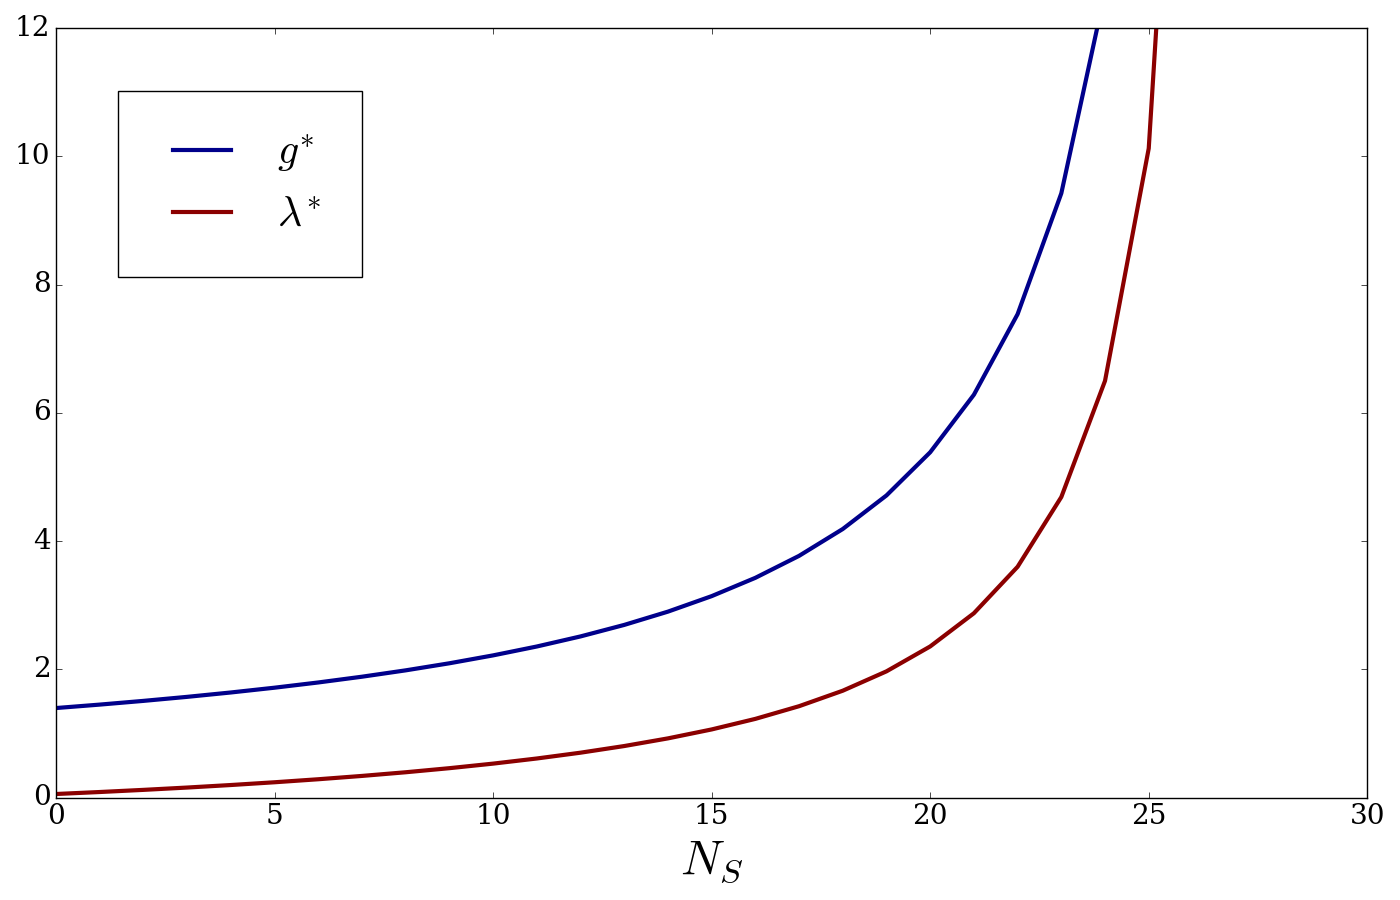
\includegraphics[width= 0.8\textwidth]{figures/FP_scalars}
 	 \caption{Impact of scalar fields on the NGFP.}	
 \end{figure}
\end{frame}

\begin{frame}{Impact on the NGFP: Perturbative Approximation II}
	 \begin{figure}[H]
 \centering
 	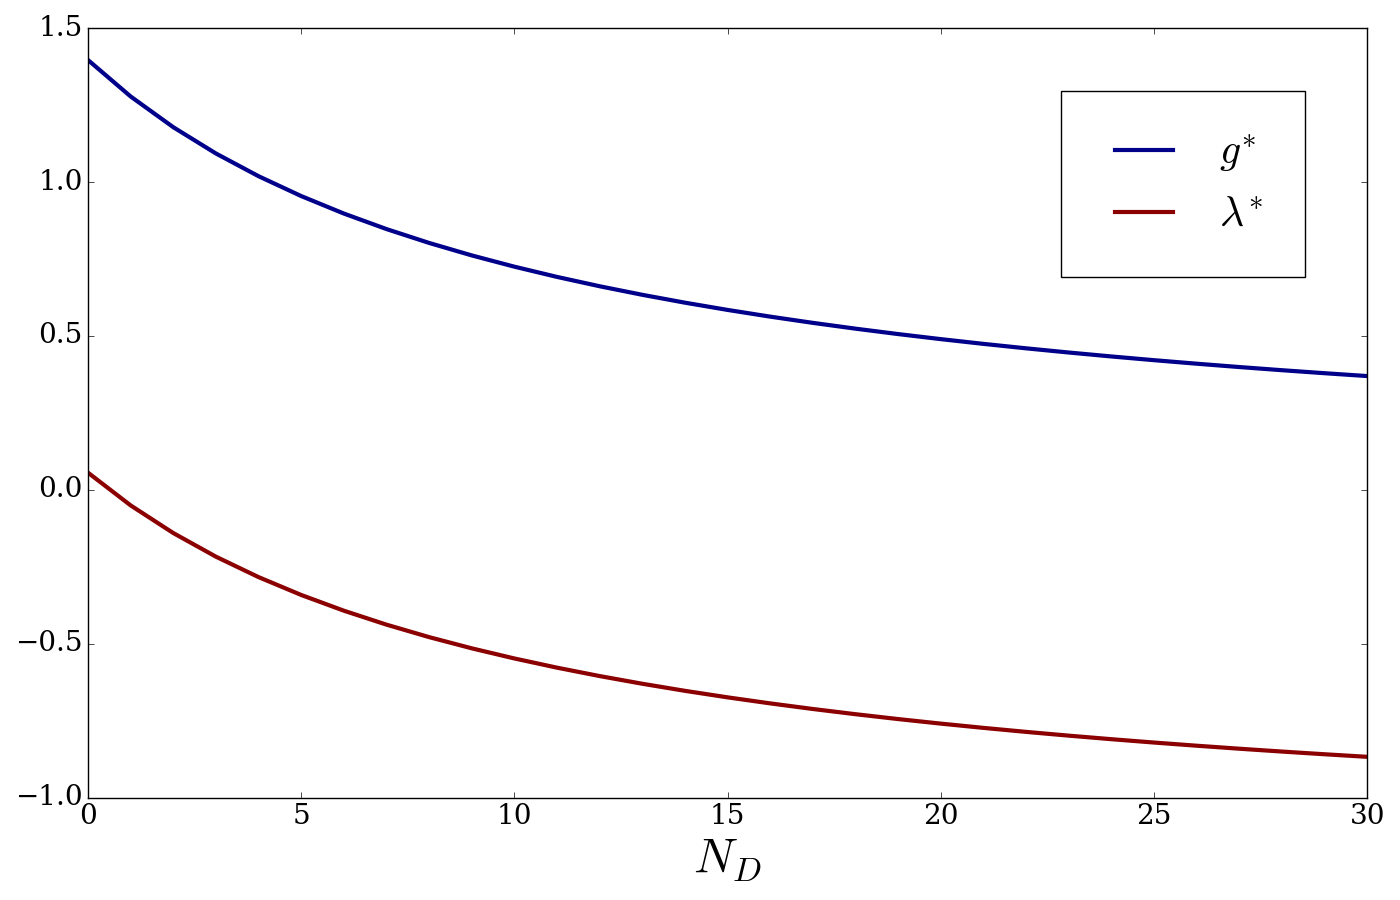
\includegraphics[width= 0.8\textwidth]{figures/FP_fermions}
 	 \caption{Impact of fermionic fields on the NGFP.}	
 \end{figure}
\end{frame}

\begin{frame}{Impact on the NGFP: Perturbative Approximation III}
	 \begin{figure}[H]
 \centering
 	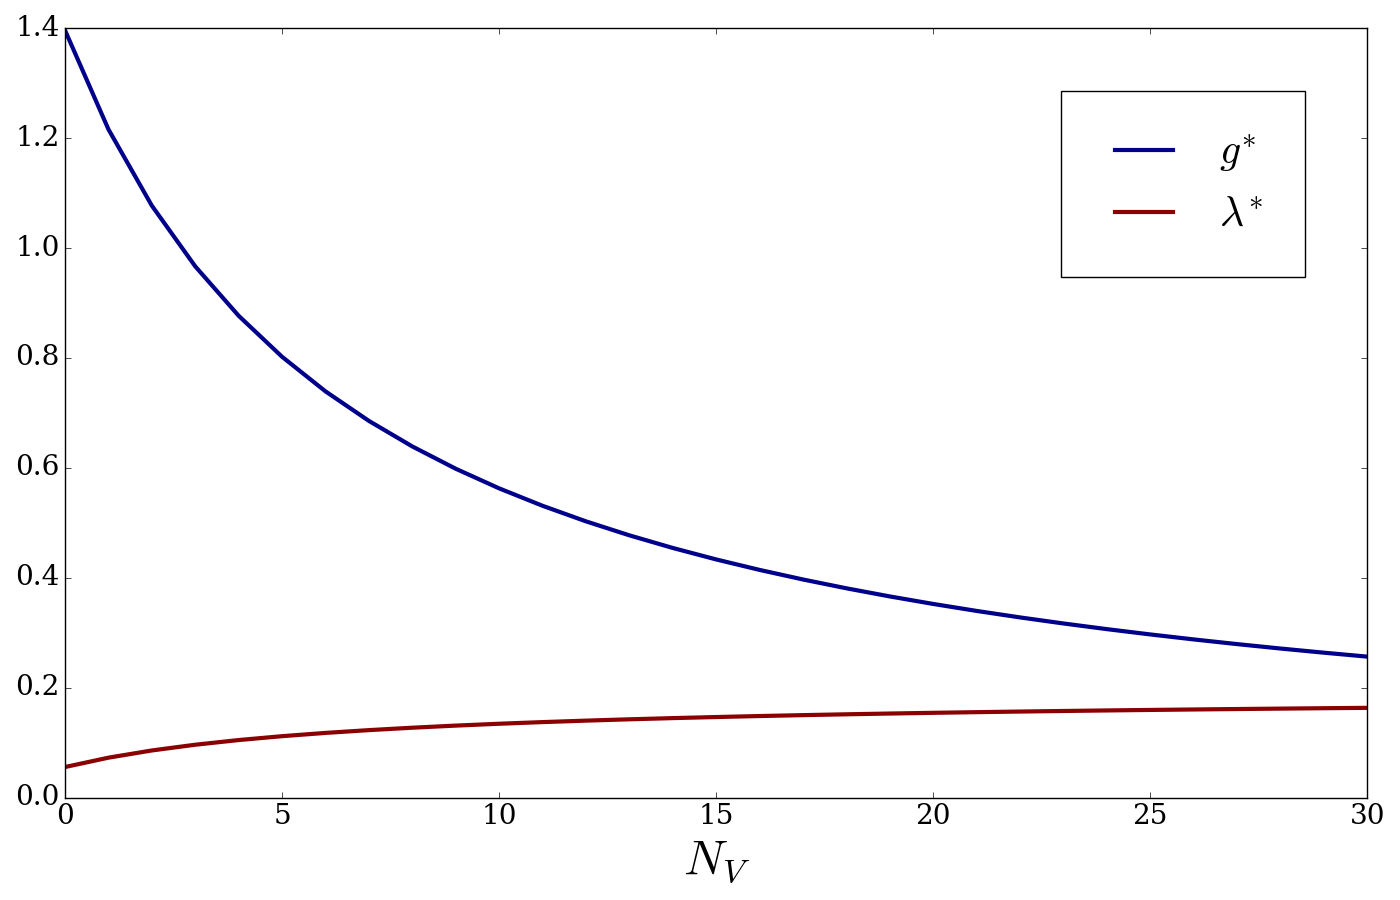
\includegraphics[width= 0.8\textwidth]{figures/FP_gauge}
 	 \caption{Impact of gauge fields on the NGFP.}	
 \end{figure}
\end{frame}

%Discussion + Conclusion
\section{Conclusion and Critical Discussion}

\begin{frame}{Conclusion}
\begin{itemize}
	\item \textbf{Pure-Gravity:} We found a NGFP at $(g_k, \lambda_k)=(0.86, 0.18)$.\vspace{0.3cm}
	\item \textbf{Gravity-Matter:} We analyzed the impact of different matter fields on the fixed point. \\\textbf{Scalars} tend to increase the fixed point values drastically after surpassing a certain amount, \textbf{fermions} decrease the values slightly and \textbf{gauge fields} leave the value of $\lambda^*$ almost unchanged, whereas the value of $g^*$ decreases rather strict.\vspace{0.3cm}
	\item \textbf{Computation:} Background field approximation has to be treated with care! Violates \textit{Nielsen Identities} and therefore \textit{background independence.}\vspace{0.3cm}
	\item \textbf{Outlook:} This work provides a suitable framework for further investigations. Next steps could involve inclusion of higher-cuvature terms or the choice of different regulators. 
\end{itemize}	
\end{frame}

\begin{frame}[shrink=20]{References}

\nocite{*}
\printbibliography

\end{frame}

\end{document}